\documentclass{beamer}

\usepackage[frenchb]{babel}
\usepackage[T1]{fontenc}
\usepackage[latin1]{inputenc}
\usepackage{amsmath}

\usetheme{Warsaw}

\begin{document}

\begin{frame}
	
	\frametitle{Procede}
	\begin{enumerate}
		\item{Conversion dans l'espace colorimetrique LAB}
		\item{Calcul des composantes de textures}
		\item{Filtrage de toutes les composantes}
		\item{Localisation des arêtes}
		\item{Sommation des composantes}
		\item{Conversion en image binaire (seuillage)}
		\item{Fermeture et squeletisation de l'image binaire}
		\item{Approximation affine des contours}
	\end{enumerate}
	
\end{frame}

\begin{frame}

	\frametitle{LAB}
	$$L = \frac{R + G + B}{3}$$
	$$A = \frac{G - R + 255}{2}$$
	$$B = \frac{G - B + 255}{2}$$

\end{frame}

\begin{frame}

	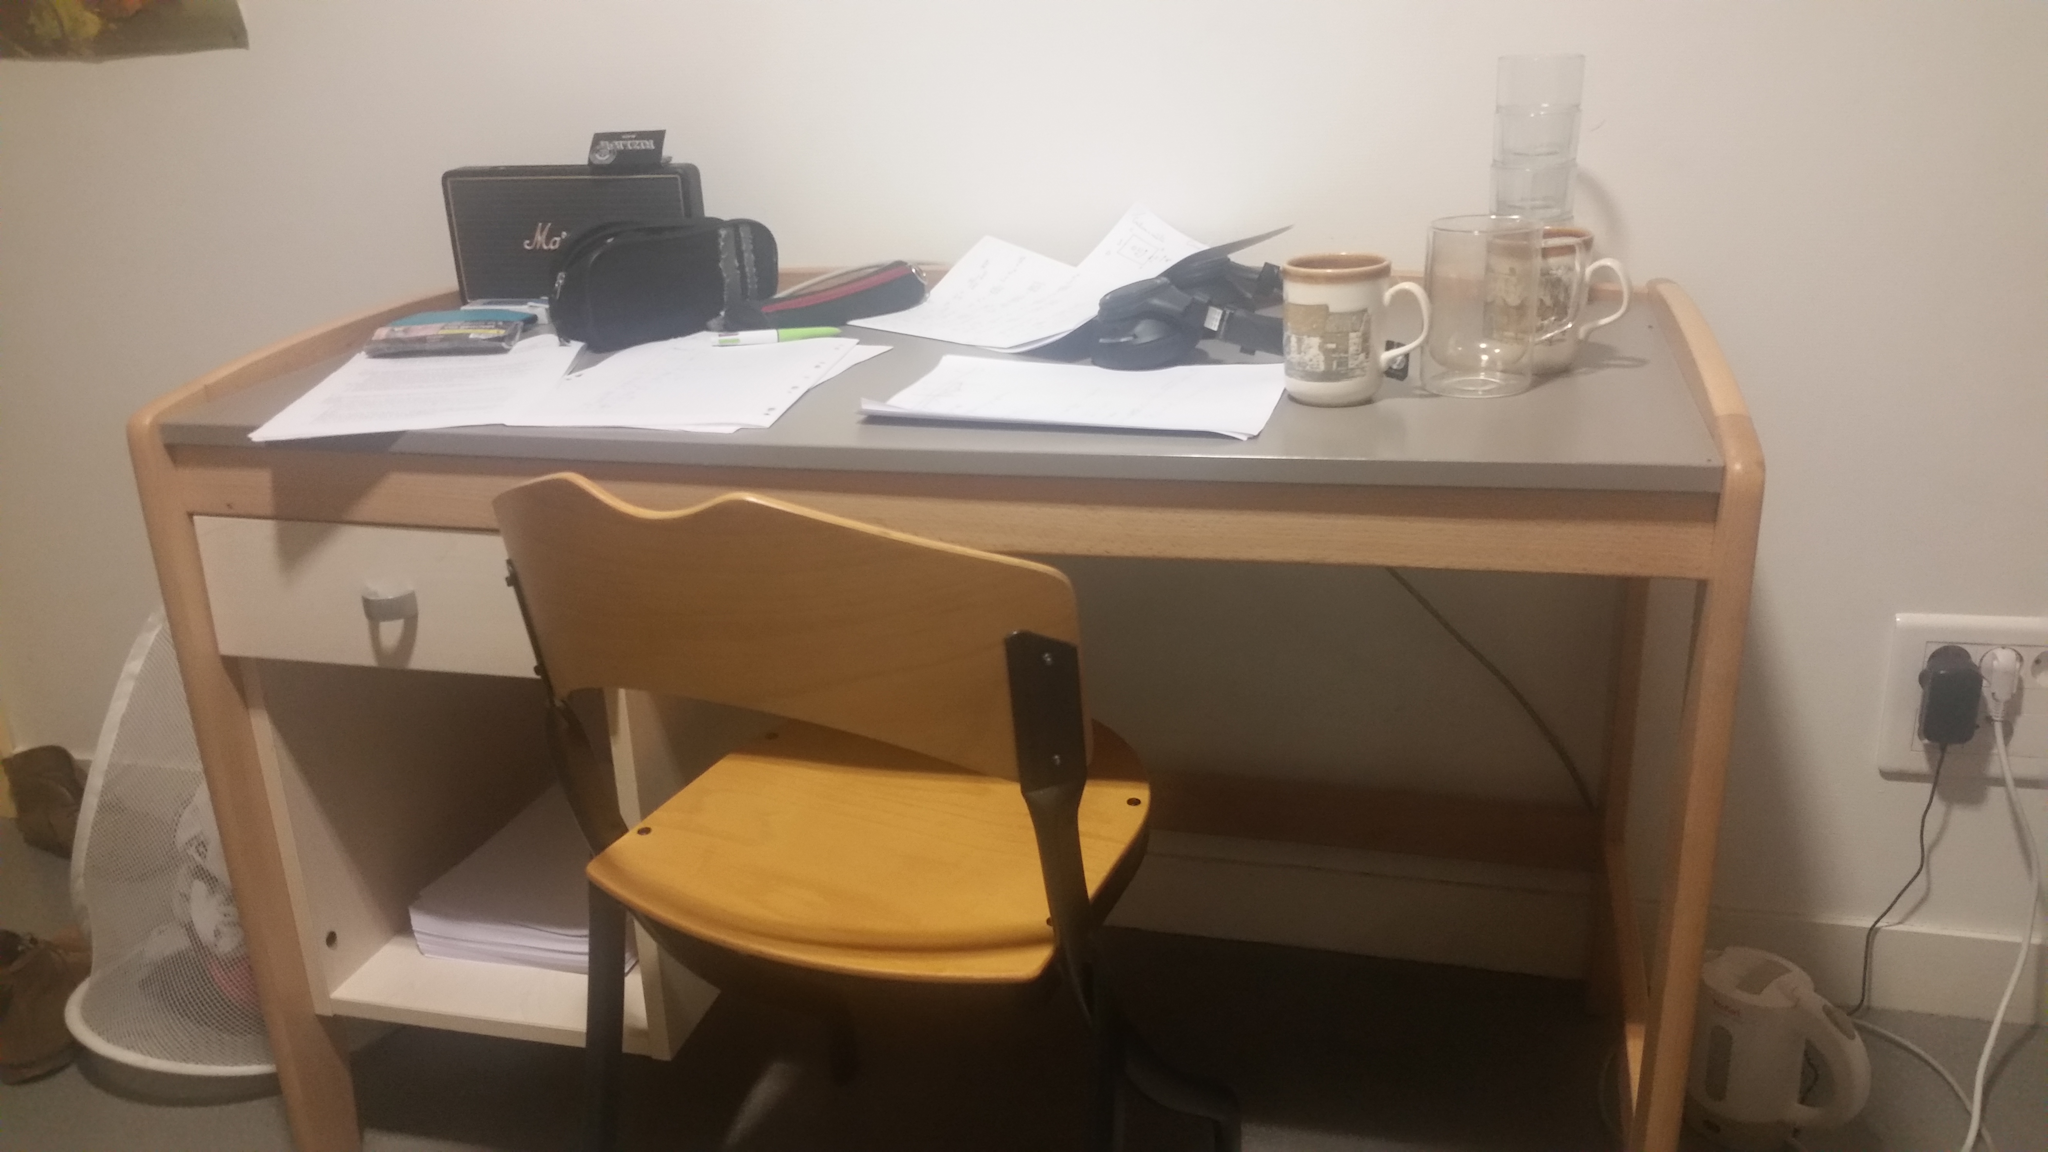
\includegraphics[width = 5cm]{bureau.png} 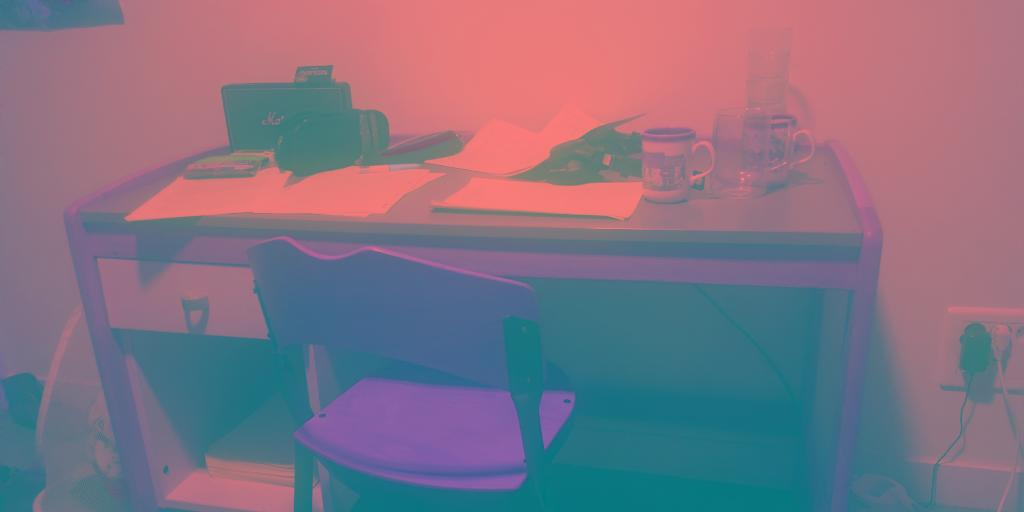
\includegraphics[width = 5cm]{bureau_lab.jpg}

\end{frame}

\begin{frame}

	\frametitle{Transformee de Fourier}
	$$F(u)(s) = \int_a^b e^{2i\pi sx} \cdot u(x) \, \mathrm dx$$
	$$FD(u)(s) = \sum_{k = 0}^{k = N} e^{2i\pi kx} \cdot u{x}$$

\end{frame}

\end{document}
